%%
%% GPW2026 Extended Abstract (下書き) -- ゲームプログラミングワークショップ
%% ベース: gi58/draft.tex (IPSJ SIG-GI58) のスタイルを流用。
%% 制約: A4縦, 2段組, 10pt以上, PDF 2ページ以内。
%%
%% TODO (要更新): 下の \newcommand 群は速報値(seed42のみ)。
%%   bearでのA1d1 5シード分完走後、scripts/analyze_cluster_switch.py と
%%   scripts/analyze_a9_validity.py を再実行し、数値を差し替えること。
%%   差し替え箇所はこの \newcommand 定義だけでよい設計にしてある。
%%

\documentclass[submit,techrep,noauthor]{ipsj}

\usepackage{graphicx}
\usepackage{latexsym}
\usepackage{amsmath,amssymb}
\usepackage{url}

\def\Underline{\setbox0\hbox\bgroup\let\\\endUnderline}
\def\endUnderline{\vphantom{y}\egroup\smash{\underline{\box0}}\\}
\def\|{\verb|}

%% ===== 数値プレースホルダ (要・実験完了後の更新) =====
% run50v2 regret (P=200, 5seed, 修正木, commit ebb5f80)
\newcommand{\regretAone}{0.514}
\newcommand{\regretAtwo}{0.506}
\newcommand{\regretAfive}{0.505}
\newcommand{\regretAseven}{0.502}
\newcommand{\regretAeight}{0.511}
\newcommand{\regretAnine}{0.508}
\newcommand{\friedmanP}{0.88}
% A9 vs A2 head-to-head (run50v2)
\newcommand{\aNineVsAtwoDq}{-0.002}
% A9 クラスタ価値の妥当性 (5seed, commit f0cb2f6)
\newcommand{\rhoCluster}{0.49}
\newcommand{\rhoCandidate}{0.30}
% クラスタ乗り換え分析 (現状 seed42速報値、要5seed化)
\newcommand{\switchEndgame}{55\%}
\newcommand{\switchMidgame}{90\%}
\newcommand{\switchOpening}{100\%}
\newcommand{\agreeEndgame}{31\%}
\newcommand{\agreeMidgame}{9\%}
\newcommand{\agreeOpening}{7\%}

\begin{document}

\title{デジタルカーリングにおけるMCTS候補手削減のための\\価値考慮型クラスタリングとその分析的応用}

\etitle{Value-Aware Clustering for Action Space Reduction \\ and Its Analytical Use in MCTS for Digital Curling}

\affiliate{MU}{明治大学\\
Meiji University}

\author{仲 亜斗夢}{Atomu Naka}{MU}[ce265004@meiji.ac.jp]
\author{横山 大作}{Daisaku Yokoyama}{MU}[dyokoyama@meiji.ac.jp]

\begin{abstract}
デジタルカーリングにおけるモンテカルロ木探索(MCTS)では，連続な行動空間から生成した多数の候補手を，結果盤面の類似性に基づく階層的クラスタリングにより削減する手法(Proposed)が検討されてきた．
本研究ではまず，Proposedの代表手選出(盤面的中心性のみに基づく)に得点期待値を組み込んだ手法ClusterValueを提案し，性能を損なわないことを確認する．
その上で，\textbf{クラスタリングを適用したMCTSにおいて候補手やその構造がどのように振る舞うか}を主眼に分析を行った．
具体的には，(i)結果盤面によるクラスタリングが候補手を盤面上のどのようなエリアへ分類するか，(ii)探索深さ(depth1とdepth3)を変えた際に選択される手がいつ・どのように変化するか，(iii)その変化がクラスタ構造上ではどう現れるかを調べた．
結果，深さによる手の変化は残り手数の少ない終盤に集中し，そのほとんどは同一クラスタ内の微調整ではなく複数候補を含む別クラスタ(戦術)への乗り換えであることが明らかになった．
また，結果盤面に基づくクラスタは得点期待値の観点で意味のあるエリアに対応しており，盤面の戦略的な見取り図(エリア価値マップ)として提示できることを示した．
これらの知見は，一手を投じた後の盤面類似性に基づくクラスタリングにより，MCTS全体で調べるべき候補手をエリア単位で効率的に絞り込める可能性を示唆する．
\end{abstract}

\maketitle

%% ======================================================================
\section{はじめに}

デジタルカーリング\cite{dc3}は，連続行動空間と実行時ノイズによる確率的不確定性を併せ持つ戦略ゲームであり，MCTSを用いた候補手選択には計算コストの課題がある．
先行研究\cite{owatari2016,kato2016}やわれわれの既報\cite{naka_gi58}では，候補手生成後の結果盤面に対して階層的クラスタリングを適用し，各クラスタの代表手のみをMCTSの子ノードとして残すことで探索対象を削減する手法(以下Proposed)を検討してきた．

しかし，Proposedの代表手選出は各クラスタ内で盤面的に最も中心的な候補(medoid)を機械的に選ぶのみであり，得点の観点からの手の良し悪しを一切考慮していない．
このため，同一クラスタ内に得点期待値の高い候補と低い候補が混在する場合，代表手が必ずしも有望な手にならないという課題があった．
実際に，等予算下でのregret評価(選んだ手と真の最良手との得点期待値差)において，Proposedはクラスタリングを行わずランダムに候補を間引く手法と有意差がなく，クラスタリングによる寄与が確認できなかった．

本研究では，まずこの課題に対し，クラスタの表現(結果盤面の類似性)は維持したまま，代表手の選出規則にのみ得点期待値を組み込む手法ClusterValueを提案し，性能を損なわないことを確認する．
その上で本研究の主眼として，\textbf{クラスタリングを適用したMCTSにおいて候補手やクラスタ構造がどのように振る舞うか}に着目する．
具体的には，クラスタリングが候補手を意味のあるエリアへどう分類するか，また探索深さを変えた際に手とクラスタ構造がどのように変化するかを分析し，結果盤面に基づくクラスタリングによる候補削減の可能性を明らかにする．

%% ======================================================================
\section{提案手法: ClusterValue}

ClusterValueは，MCTSのルートノードにおいて以下の手順で候補手を選別する．
(1) 各候補手について，安価なロールアウト(既定3回)により得点期待値$\hat{E}[\mathrm{score}]$を推定する．
(2) Proposedと同一の距離関数・階層的クラスタリング(平均連結法)により，結果盤面を基準に候補手をクラスタへ分割する．
(3) 各クラスタの価値を，メンバー候補の$\hat{E}[\mathrm{score}]$の平均値として定義する．クラスタ単位で平均を取ることで，個々の候補の推定に含まれる分散を低減できる．
(4) 価値上位$K$個のクラスタを採用し，各クラスタ内で$\hat{E}[\mathrm{score}]$が最大の候補を代表手としてMCTSの子ノードに割り当てる．全体の最良候補が属するクラスタは，価値順位によらず必ず採用する．

Proposedとの差異は(3)(4)のみであり，探索木の構造・ロールアウト方策・木の深さ以降の展開は共通である．
したがって両手法の比較は，「代表手選出規則を盤面中心性から得点期待値ベースへ変更した効果」を単離して評価できる．

%% ======================================================================
\section{実験: クラスタリングを適用したMCTSの振る舞い}

\subsection{実験設定と前提の確認}
自己対戦から抽出した50局面$\times$5乱数系列に対し，AllGrid(全候補を子ノードとする基準手法，A1)，Proposed(A2)，ClusterValue(A9，提案手法)を等物理シミュレーション予算下で評価した．
各候補を実行ノイズ込みで$K{=}200$回再試行する審判機構によりregret(選択手と真の最良手との得点期待値差)を求めたところ，A1: \regretAone，A2: \regretAtwo，\textbf{A9: \regretAnine}であり，Friedman検定でも有意差は見られなかった($p={\friedmanP}$)．
すなわち\textbf{ClusterValueは性能を損なうことなくProposedの代表手選出を改善できる}ことを確認したうえで，以下ではこのクラスタ構造を用いて，候補手の分類と探索深さの影響を分析する．

\subsection{クラスタリングによる候補手の意味的分類}
図\ref{fig:areamap}に，ある局面でClusterValueが生成したクラスタを示す．
結果盤面の類似性に基づくクラスタは，投球後の石の配置が近い候補手をまとめる傾向があり，各クラスタに得点期待値を対応付けることで，盤面上のどのエリアへの投球が有望かを可視化できる(エリア価値マップ)．

\begin{figure}[tb]
\centering
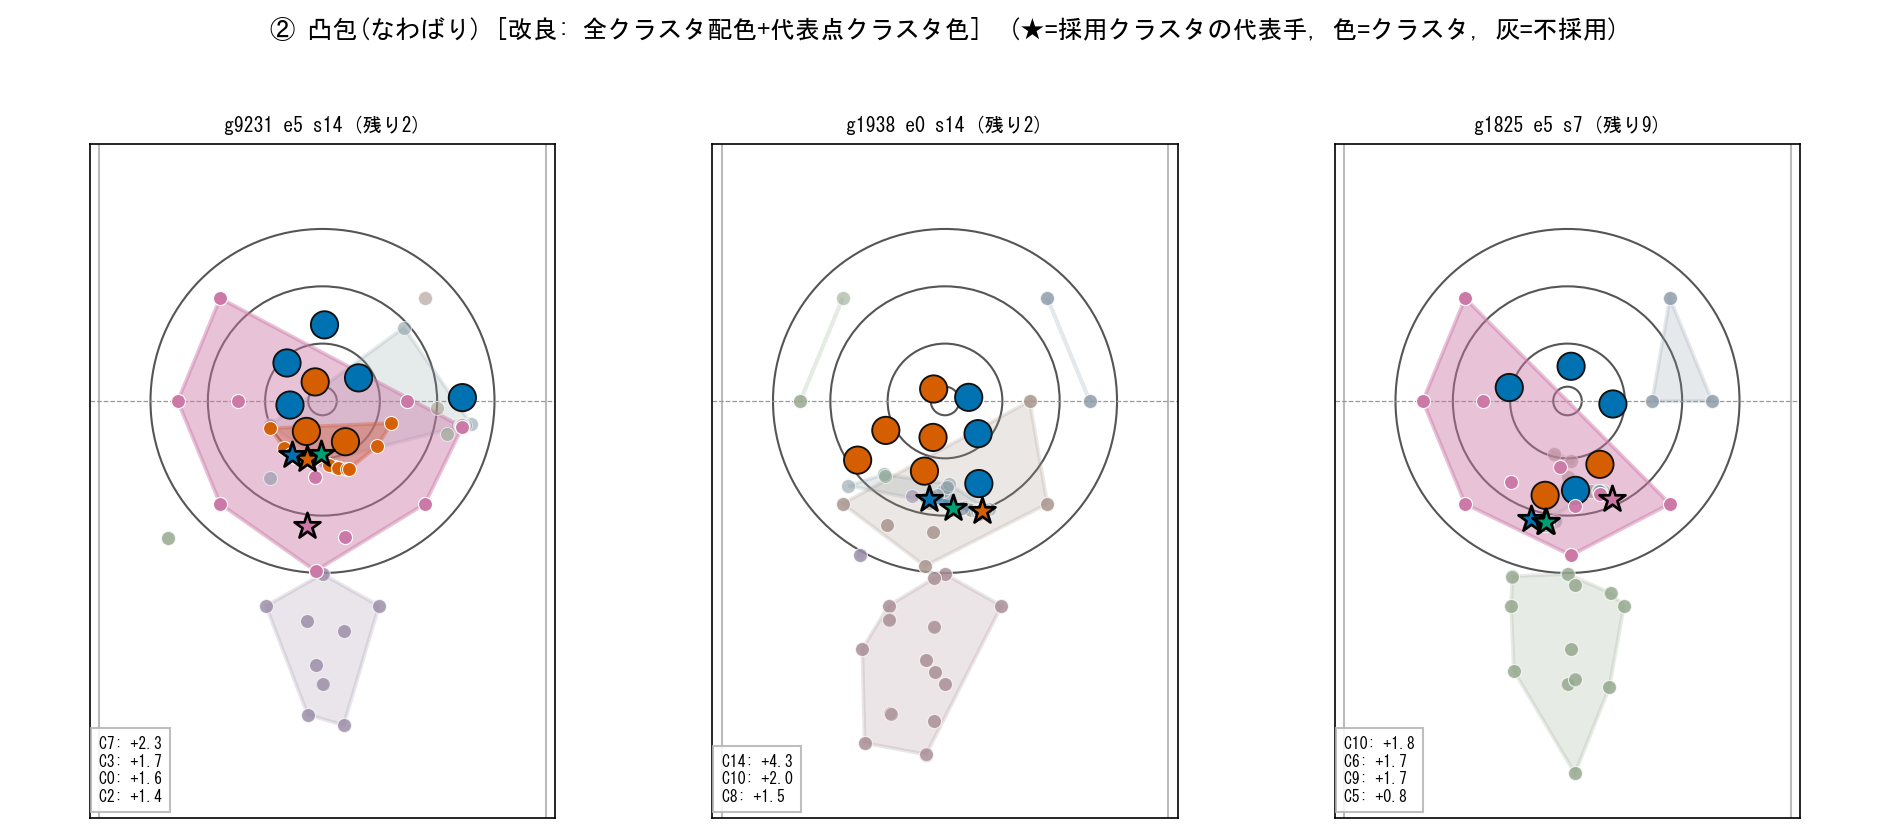
\includegraphics[width=\columnwidth, bb=0 0 907 403]{figures/area_map_B_hull_draft.png}
\caption{エリア価値マップの例．採用クラスタを色分けした凸包で表示し(灰色は不採用クラスタ)，星印は各クラスタの代表手，数値はクラスタの得点期待値．}
\label{fig:areamap}
\end{figure}

このクラスタ分類が単なる次元削減ではなく戦略的に意味のある区分けになっているかを，クラスタ価値($\hat{E}[\mathrm{score}]$の平均)と審判値とのSpearman順位相関で検証した．
候補単位の相関(中央値$\rho\fallingdotseq\rhoCandidate$)に対し，クラスタ単位の相関は中央値$\rho\fallingdotseq\rhoCluster$であり，\textbf{5乱数系列すべてで}クラスタ単位の方が高い精度を示した．
個々の候補の推定に含まれる分散が，クラスタ内で平均を取ることで低減された結果と考えられる．

\subsection{探索深さによる手の変化はいつ起こるか}
探索深さを1(d1)から3(d3)に変えると，MCTSが選ぶ手はどう変わるか，またそれはいつ起こるかを調べた．
残り手数を終盤(2--4手)・中盤(5--8手)・序盤(9手以上)の3区分に分け，d1とd3の選択一致率を比較したところ，序盤\agreeOpening，中盤\agreeMidgame，終盤\agreeEndgame であった(図\ref{fig:agreement})．
\textbf{手の変化は残り手数の少ない終盤に集中しており}，これは木がエンドの最終局面に到達し探索の効果が最も強く現れる範囲が終盤に限られるためと考えられる．

\begin{figure}[tb]
\centering
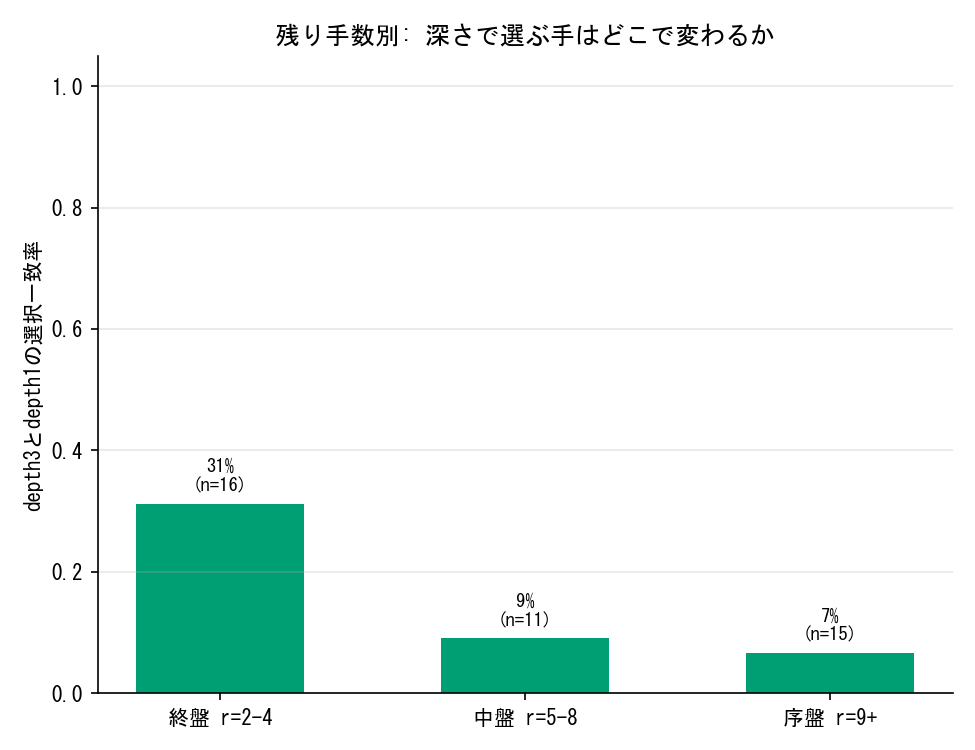
\includegraphics[width=\columnwidth, bb=0 0 468 360]{figures/agreement_by_phase_draft_seed42.png}
\caption{残り手数の区分別，depth3とdepth1の選択一致率(速報値)．終盤ほど一致率が低い．}
\label{fig:agreement}
\end{figure}

\subsection{手の変化に伴うクラスタの変化}
手の選択が分かれた局面について，d1の手とd3の手が同一クラスタに属するか，別クラスタに属するかを調べた(図\ref{fig:switch})．
別クラスタへの乗り換えの割合は終盤\switchEndgame，中盤\switchMidgame，序盤\switchOpening であり，\textbf{手の変化の多くは同一クラスタ内の微調整ではなく，別の戦術グループへの乗り換えとして生じている}．
乗り換え元・先のクラスタはいずれも複数候補を含んでおり(単独候補への収束ではない)，個々の候補ではなく戦術グループ単位で選択が再考されていることを裏付ける．
また終盤の乗り換えでは，石を排除するヒットからガード・ドローへの変化が多く観察され，浅い探索では見えなかった選択肢が深い探索によって浮上する様子が確認された．

\begin{figure}[tb]
\centering
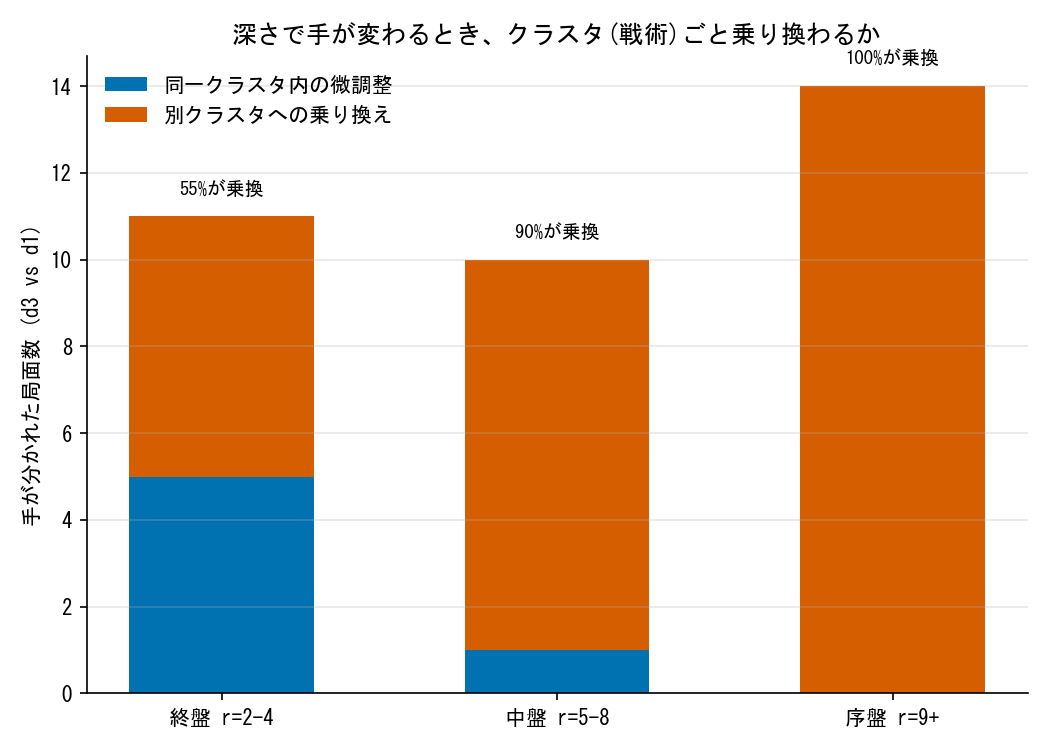
\includegraphics[width=\columnwidth, bb=0 0 504 360]{figures/cluster_switch_draft_seed42.png}
\caption{深さで手が変わる際の，クラスタ単位での乗り換え割合(残り手数の区分別，速報値)．}
\label{fig:switch}
\end{figure}

%% ======================================================================
\section{おわりに}

本研究では，結果盤面の類似性に基づくクラスタリングを用いたMCTSにおいて，候補手やクラスタ構造がどのように振る舞うかを分析した．
まずClusterValueにより，性能を損なうことなくProposedの代表手選出(価値盲目なmedoid選択)を改善できることを確認した．
その上で，(i)候補手は得点期待値の観点で意味のあるエリアへ分類されること，(ii)探索深さの効果は終盤に集中し，そのほとんどが個々の候補ではなく戦術グループ単位の乗り換えとして現れることを明らかにした．
これらの結果は，一手を投じた後の盤面類似性に基づくクラスタリングにより，MCTS全体で調べるべき候補手をエリア単位で効率的に絞り込める可能性を示唆する．

現状の分析は事前に用意した局面集合に対するオフライン評価にとどまり，時間制約下での実戦的な対局には未対応である．
今後は，本研究で得られた知見(探索資源を終盤エリアへ重点配分する等)を反映した実装を行い，過去の大会優勝プログラムとの対戦を通じて実戦的な有効性を検証したい．

\begin{thebibliography}{10}

\bibitem{owatari2016}
大渡勝己，田中哲朗：
モンテカルロ木探索によるデジタルカーリングAI，
第21回ゲームプログラミングワークショップ, pp. 180--187 (2016).

\bibitem{kato2016}
加藤修，飯塚博幸, 山本雅人：
不確定性を含むデジタルカーリングにおけるゲーム木探索，
情報処理学会論文誌，Vol.2016-GI-57, No.11, pp.~2354--2364 (2016).

\bibitem{dc3}
北清勇磨，岡田雷太，伊藤毅志：
デジタルカーリングサーバーの提案と紹介，
情報処理学会研究報告. GI, [ゲーム情報学] 2014(2)，pp.~1--5 (2014).

\bibitem{naka_gi58}
仲 亜斗夢，横山 大作：
デジタルカーリングにおけるMCTS候補手削減のためのクラスタリング適用の試み，
情報処理学会研究報告. GI, [ゲーム情報学] 2026-GI-58 (2026).

\end{thebibliography}

\end{document}
